\chapter{Reinforcement learning and Self play approach}
\section{Introduction}
\section{Reinforcement Learning}
\subsection{Definition}
\citeauthor{RLIntroduction} \cite[Chapter.~1]{RLIntroduction} gave an excellent in-depth definition, which not only defines what \acrfull{rl} is, but also compare it with other \acrfull{ml} methods.
\newline We will summarize it as follow:
\begin{definition}
	
\end{definition}
\begin{figure}
	\centering
	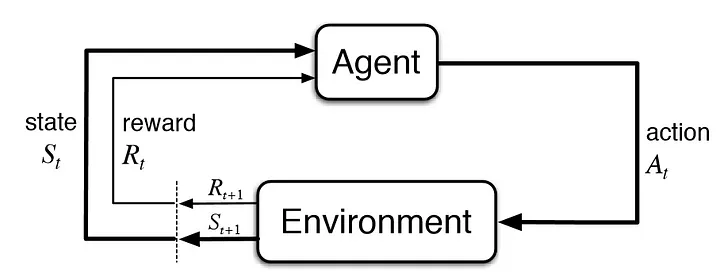
\includegraphics[width= 0.8\textwidth]{Figures/RLDiagram.png}
	\caption{A Reinforcement Learning system}
\end{figure}
\subsection{Theory}
\subsubsection{Single Agent}
In most settings, the theory of \acrshort{rl} deals with environments where we would like to optimize a single agent. This is called single agent \acrshort{rl}. This is usually modeled within a \acrfull{mdp}
\parencites[chapter.~3]{RLIntroduction}[chapter.]~23]{AIModernApproach}

Now, the sole problem is the agent itself may or maynot know the model\footnote{In this particular context, a model of the \acrshort{mdp} is the representation of all transitions, their rewards, and the transition probabilities. That is the complete knowledge of the \acrshort{mdp}. This has nothing to do with our meaning of model.} of the \acrshort{mdp}. Thus there are mainly two approaches:
\begin{itemize}
	\item \textbf{Model-based \acrshort{rl}}.
	\item \textbf{Model-free \acrshort{rl}}. 
\end{itemize}

Single agent \acrshort{rl} applies when we want to find the best counter strategy of player $\Opt\in\PlayerSet$ in a \acrshort{mpg}. Model-based \acrshort{rl} applies when $\Opt$'s strategy is deterministic\footnote{For the deterministic case, \acrshort{rl} is an overkill. We can fallback to negative cycle finding.} or fractional. If $\Opt$'s strategy is complicated or unknown, we can only use Model-free \acrshort{rl} methods.

While our ultimate objective is a model that plays good enough irrespective of the opponent's strategy, our implementation does support for \acrshort{rl}-based strategy countering, albeit it does need retraining for every \acrshort{mpg} instance.

\subsubsection{Multi Agent}
When we have multiple agents with potentially conflicting objectives, we call this multi-agent \acrshort{rl}.

As the single agent case, each agent in the \acrshort{sg} may or may not know the the underlying model\footnote{Model as in the \acrshort{mdp} sense.}.

In our case, a \acrshort{mpg} can be modeled in the \acrshort{rl} setting as a turn-based, two-player, zero-sum \acrfull{sg}\footnote{Also known as Markov Game} \cite{StochasticGames}.

We will use the \acrshort{sg} formalism for the self-playing part.
\subsection{\acrshort{rl} formalisation of a \acrshort{mpg}}
To formalise a \acrshort{mpg} in \acrshort{rl} setting, we have two formalisms. Before diving into that, we will use the \acrshort{mpg} definition in section \ref{section:Formalisation:MPG}:
\begin{equation*}
	G=(\VertexSet,\EdgeSet,W,s,p)
\end{equation*}

\subsubsection{Instance based formalism}
In this formalism, we the \acrshort{sg} is directly defined by the \acrshort{mpg}.

That is, th

\subsubsection{Global formalism}
In this formalism, we will augment the \acrshort{sg} to account to the space of all \acrshortpl{mpg}.

This will require the following definition:
\begin{definition}
	The set of all \acrshortpl{mpg}, denoted by $\mathbb{M}$ is the set generated by $G=(\VertexSet,\EdgeSet,W,\PlayerSet,s,p)$ where:
	\begin{enumerate}
		\item $\varnothing\subsetneq V \subset_{\text{finite}} \mathbb{N}$
		\item $E \subseteq V\times V$ with the sinkless requirement:
		\begin{equation*}
			\forall u \in V,\quad \Adj u \neq \varnothing
		\end{equation*}
		\item $W\in\mathscr{F}(E,[-1,1])$
		\item $s\in \VertexSet.$
		\item $p\in \PlayerSet$
	\end{enumerate}
\end{definition}
	This set contains all \acrshortpl{mpg} up to isomorphism and positive rescaling.
	
	In this sense, we can play $G$ in $\mathbb{M}$ as follow:
	\begin{itemize}
		\item We set $G\in \mathbb{M}$ as the starting state.
		\item Let $G=(\VertexSet,\EdgeSet,W,\PlayerSet,s,\Opt)$ be the current node, then $\Opt\in\PlayerSet$ is the current player, his available actions are $\Adj s$
		\item Suppose that $\Opt$ chose action $t\in \Adj s,$ then he gets a payoff of $W(s,t),$ and the state transitions to $G'=(\VertexSet,\EdgeSet,W,\PlayerSet,t,\bar{\Opt})$
	\end{itemize}
	In fact, the game that we have just proposed is the same as the following \acrshort{mpg} $\mathscr{G}=(\mathbb{M},\mathbb{E},\mathbb{W},\VertexSet,G,p)$ with:
	\begin{align*}
		\mathbb{E}&=\left\{(\VertexSet,\EdgeSet,W,\PlayerSet,s,\Opt)\rightarrow (\VertexSet,\EdgeSet,W,\PlayerSet,t,\bar{\Opt})/\quad (s,t) \in E\right\} \\
		\forall G\rightarrow G',\quad \mathbb{W}(G,G')&=W(s,t) \quad \text{Where} \ \begin{cases}
			s & \text{is the starting vertex of} \ G \\
			t & \text{is the starting vertex of} \ G'
		\end{cases} 
	\end{align*} 
	Now, it is trivial to see that the \acrshort{mpg} $\mathscr{G}$ is equivalent to $G,$ and here we put all this theory into effect: \textbf{The \acrshort{rl} methods will be done in $\mathscr{G}$ instead of $G$.}
	
	\subsection{Benefits of global formalism}
	At first glance, it seems that we have only complicated the matter. In fact, this is justified as we can only effectively apply function approximation methods \acrshort{rl} using the global formalism.
	
	To clarify our point, we recall that in chapter \ref{section:ModelDesign}, we designed a model $\mathcal{M}_\Theta$ that takes a \acrshort{mpg} $G$ and outputs a strategy $\Pi_\Theta$ and an evaluation $v_\Theta.$ We will use \acrshort{rl} to refine $\Theta$ so that: 
	\begin{itemize}
		\item $v_\Theta(G)$ approaches the value of the game\footnote{The definition is stated in section} $v(G).$
		\item $\Pi_\Theta(G)$ approaches an optimal strategy $\Pi$ of game $G.$
	\end{itemize}
	Now, with the right choice of \acrshort{rl} algorithm, we expect that for any close enough\footnote{To formalise this idea, we need to define a metric space in $\mathbb{G}.$ This is beyond the scope of this report, but the point still holds.} game $G':$
	\begin{itemize}
		\item $v_\Theta(G')$ will also approach the value of the game $v(G').$
		\item $\Pi_\Theta(G')$ will also approach an optimal strategy $\Pi$ of game $G'.$
	\end{itemize}
	This is crucial: \textbf{We are training $\mathcal{M}_{\Theta}$ using \acrshort{rl} so that it generalises to any \acrshort{mpg}.}
	
	In contrast, if we just use the instance based formalism, the underlying model can only take the current position as information, and thus it does only generalises to solving the same game, but with only varying starting positions.
	\subsection{Generating random \acrshortpl{mpg}}
	This is the last thing to be addressed before implementing the self-playing pipeline.
	
	To expect our model to generalises well to any \acrshort{mpg}. We should generate the games using a suitable distribution. To do that, we introduced two additional distributions:
	\subsubsection{$\mathcal{D}^\bullet_{p,\text{US}}$ distribution}
	\begin{itemize}
		\item Let $\mathcal{N}$ be a non-empty finite subset of $\mathbb{N}.$ 
		\item Let $\mathcal{P}$ be a mesurable subset of $[0,1].$
		\item For a mesurable set $S,$ we will denote by $\mathcal{U}(S)$ the uniform distribution on $S.$
	\end{itemize}
	The $\mathcal{D}^\bullet_{p,\text{US}}(\mathcal{N},\mathcal{P})$ is a mixture distribution defined as follow:
	\begin{equation*}
		\mathcal{D}^\bullet_{p,\text{US}}(\mathcal{N},\mathcal{P}) = \mathcal{D}^\bullet(N,P) \quad \text{where}\ \begin{cases}
			N &\sim \mathcal{U}(\mathcal{N}) \\
			P &\sim \mathcal{U}(\mathcal{P})
		\end{cases}
	\end{equation*}
	To sample an element from $\mathcal{D}^\bullet_{p,\text{US}}(\mathcal{N},\mathcal{P})$:
	\begin{enumerate}
		\item Select the graph size $N\in\mathcal{N}$ uniformly at random.
		\item Select the edge probability $p\in\mathcal{P}$ uniformly at random.
		\item Build $G\sim \mathcal{D}^\bullet(N,P)$ using algorithm \ref{alg:Dnp_Fast} and degree rejection method defined at section \ref{section:Dataset:Sinkless:DegreeRejection}.
			
	\end{enumerate} 
	
	\subsubsection{$\mathcal{D}^\bullet_{c,\text{US}}$ distribution}
	\begin{itemize}
		\item Let $\mathcal{N}$ be a non-empty finite subset of $\mathbb{N}.$ 
		\item Let $\mathcal{C}$ be a non-empty finite subset of $\mathbb{N}.$
	\end{itemize}
	The $\mathcal{D}^\bullet_{c,\text{US}}(\mathcal{N},\mathcal{C})$ is a mixture distribution defined as follow:
	\begin{equation*}
		\mathcal{D}^\bullet_{c,\text{US}}(\mathcal{N},\mathcal{C}) = \mathcal{D}^\bullet(N,\tfrac{C}{N}) \quad \text{where}\ \begin{cases}
			N &\sim \mathcal{U}(\mathcal{N}) \\
			C &\sim \mathcal{U}(\mathcal{C})
		\end{cases}
	\end{equation*}
		To sample an element from $\mathcal{D}^\bullet_{c,\text{US}}(\mathcal{N},\mathcal{C})$:
	\begin{enumerate}
		\item Select the graph size $N\in\mathcal{N}$ uniformly at random.
		\item Select the expected degree $c\in\mathcal{C}$ uniformly at random.
		\item Build $G\sim \mathcal{D}^\bullet(N,\tfrac{C}{N})$ using algorithm \ref{alg:Dnp_Fast} and degree rejection method defined at section \ref{section:Dataset:Sinkless:DegreeRejection}.
	\end{enumerate} 
\subsubsection{Importance}
In chapter \ref{section:Dataset}, we designed and implemented a graph generation pipeline, then a graph annotation pipeline for dense graphs and later sparse graphs.

Both datasets $\mathcal{D}^\text{dense}$ and $\mathcal{D}^\text{sparse}$ contain the evaluation of each game and its respective optimal strategy. We can use both datasets for evaluation purposes, and for that we will make sure that our learns from the same distribution.

Following our implementation in chapter \ref{section:Dataset}: 
\begin{itemize}
	\item Each generated dense graph follow $\mathcal{D}^\bullet_{p,\text{US}}(\mathcal{N},\mathcal{P}).$ with $\mathcal{N}$ and $\mathcal{P}$ defined on section \ref{section:MPG:Generation:Distribution}, at the \textbf{Dense Graphs} paragraph.
	\item Each generated sparse graph follow $\mathcal{D}^\bullet_{c,\text{US}}(\mathcal{N},\mathcal{C})$ with $\mathcal{N}$ and $\mathcal{C}$ defined on section \ref{section:MPG:Generation:Distribution}, at the \textbf{Sparse Graphs} paragraph.
\end{itemize} 
	
\subsection{Considered \acrshort{rl} algorithm}
Now, all the technicalities about the formalisation of \acrshort{mpg} in \acrshort{rl} setting are resolved. Also, we have a complete model $\mathcal{M}$ as a result of chapter \ref{section:ModelDesign}.

The remaining part is the choice of the \acrshort{rl} itself. As hinted by previous sections, we will implement a self-playing system based on Alpha Zero \cite{AlphaZero}.

This system will indefinitevely:
\begin{itemize}
	\item Generate random instances of a \acrshort{mpg}, and annotate them with the model $\mathcal{M}_{\Theta}$ using self-play.
	\item Sample a dataset $\mathcal{D}$ from the generated annotated games, and fit the model $\mathcal{M}_{\Theta}$ to get a refined model $\mathcal{M}_{\Theta'}.$
	\item Evaluate the model against a fixed set of opponents.
\end{itemize}
With all that said, only the self-playing system is remaining. Thus in the upcoming sections, we will:
\begin{enumerate}
	\item Formalise the self-playing approach.
	\item Fully implement it.
	\item Deploy it in a \acrshort{hpc} cluster.
	\item Execute the whole pipeline and fine-tune the model.
\end{enumerate}
\newpage
\section{Monte Carlo Tree Search}
\acrfull{mcts} is an advanced algorithm in decision making that appeared in \citedate{MCTSOriginal}. \citeauthor{MCTSOriginal} first coined the term \acrshort{mcts} as application of Monte-Carlo methods to game-tree search \cite{MCTSOriginal}. It is an important algorithm for adversial search. that had a huge success at improving the competence of Go engines to a master level \cite{GoMaster}. This alone was a feat considering that previous state of the are alpha-beta implementations were unable to get past beginner level. 

Much development occured to \acrshort{mcts}, which made it a little hard to define. \citeauthor{RLIntroduction} gave the following definition \cite[section.~8.8]{RLIntroduction}: \textit{``\acrfull{mcts} is a planning algorithm that accumulates value estimates obtained from Monte Carlo simulations in order to successively direct simulations towards more highly-rewarded trajectories."}

This definition alone is unsatisfactory, \citeauthor{AIModernApproach} gave an intuitive explanation \cite[Section~6.4]{AIModernApproach} of how \acrfull{mcts} works for a game. And we will base this section on his work. 
 
Essentially, \acrshort{mcts} consists of the following $4$ steps:
\subsection{Selection}
Starting at the root, we choose a child following a \textbf{selection policy} $\Pi^{\text{selection}}$, and repeat the step until arriving to a leaf node.
\begin{algorithm}
	\caption{Selection algorithm for \acrshort{mcts}}\label{alg:MCTSSelection}
	\begin{algorithmic}
		\Require $r$ the root of the \acrshort{mcts}.
		\Require $\Pi^{\text{selection}}$ the current selection policy..
		\Ensure $s$ a leaf of the \acrshort{mcts}.
		\State $s\leftarrow r$
		\While{$\Not \ \text{leaf}(r)$}
			\State  $s\leftarrow \Pi^{\text{selection}}(r)$
		\EndWhile
		\State \Return $s$
	\end{algorithmic}
\end{algorithm}

\subsection{Expansion}
At the selected leaf $s$, we grow the \acrshort{mcts} by adding a new child $t$ that is a result of some action $a$ from $s.$

\begin{algorithm}
	\caption{Expansion algorithm for \acrshort{mcts}}\label{alg:MCTSExpansion}
	\begin{algorithmic}
		\Require $s$ a leaf \acrshort{mcts}.
		\Require $H$ the mean reward of each node in the \acrshort{mcts}
		\Require $T$ the number of simulations for each node in the \acrshort{mcts} 
		\Ensure $t$ a new child of $s$
		\State  $C\leftarrow \text{expand\_children}(s)$ \Comment{Generate a set of children from $s$}
		\For {$c \in C$}
			\State $T(c)\leftarrow 0$ \Comment{$c$ is currently visited $0$ times}
			\State $H(c)\leftarrow \boldsymbol{0}$ \Comment{The reward of each player at $c$ is initialized to $0$}
		\EndFor
		\State \text{$t\leftarrow \text{choose}(C)$} \Comment{Choose a child from $C$}
		\State \Return $t$
	\end{algorithmic}
\end{algorithm}

\subsection{Simulation}
Starting from the new child $t,$ we perform a complete playout, that is, we choose moves for all players according to the playout policy $\Pi^{\text{playout}}.$
\newline The generated sequence of nodes in the playout will not be recorded in the \acrshort{mcts}
\begin{algorithm}
	\caption{Simulation algorithm for \acrshort{mcts}}\label{alg:MCTSSimulation}
	\begin{algorithmic}
		\Require $t$ the new child of the \acrshort{mcts}.
		\Require $\Pi^{\text{playout}}$ the current playout policy..
		\Ensure $W$ the cumulative rewards after the playout for each player.
		\State  $s\leftarrow \text{state}(t)$ \Comment{get the current state}
		\State  $p\leftarrow \text{state}(t)$ \Comment{get the current player}
		\State $W\leftarrow \boldsymbol{0}$ 
		\While{$\Not \ \text{terminal}(s)$}
		\State  $a\leftarrow \Pi^{\text{playout}}(s,p)$
		\State $(s,p,U) \leftarrow \text{apply}(s,a)$ \Comment{Apply action $a$ at state $s$, and getting reward $U$}
		\State $W\leftarrow W+U$
		\EndWhile
		\State \Return $W$
	\end{algorithmic}
\end{algorithm}


\subsection{Backpropagation}
Once a simulation is complete, we use its result to update the all search nodes going from $t$ up to the root.
\begin{algorithm}[h]
	\caption{Backpropagation algorithm for \acrshort{mcts}}\label{alg:MCTSBackpropagation}
	\begin{algorithmic}
		\Require $t$ the new child of the \acrshort{mcts}.
		\Require $W$ the reward after the simulation.
		\Require $W'$ the cumulative reward up to node $t$
		\Require $H$ the mean reward of each node in the \acrshort{mcts}
		\Require $T$ the number of simulations for each node in the \acrshort{mcts}
		\While{$\Not \ \text{root}(s)$}
		\State $T(s)\leftarrow T(s)+1$ \Comment{Increment the number of visits of $s$}
		\State $H(s)\leftarrow H(s) - \frac{W+W'-H(s)}{T(s)}$  \Comment{Update the mean reward at $s$}
		\State $s\leftarrow \text{parent}(s)$ \Comment{Go to the parent node}
		\EndWhile
		\State \Return $W$
	\end{algorithmic}
\end{algorithm}
\FloatBarrier
\subsection{Wrapping up}
Once we have the $4$ elements of \acrshort{mcts}, the full algorithm will be just repeating these steps in order until certain desired condition is satisfied. In practice, most implementations use the following conditions for halting the  algorithm:
\begin{itemize}
	\item Execution time exceeds some threshold $T$
	\item Total number of simulations (at root) exceeds some threshold $N$
\end{itemize}

\begin{algorithm}
	\caption{\acrshort{mcts} Algorithm}\label{alg:MCTS}
	\begin{algorithmic}
		\Require $\text{state}$ some state of the game
		\Ensure An action $a\in \text{actions}(\text{state})$
		\State $r\leftarrow \text{tree}(\text{state})$
		\While {Exit condition not satisfied}
		\State $s\leftarrow \text{select}(r)$
		\State $t\leftarrow \text{expand}(s)$
		\State $W\leftarrow \text{simulate}(t)$
		\State $\text{backpropagation}(t,W)$
		\EndWhile
		\State \Return $a\leftarrow \displaystyle \argmax_{a\in \text{actions}(\text{state})}T(a)$ \Comment{Get the most visited action}
	\end{algorithmic}
\end{algorithm}
\begin{figure}
	\centering
	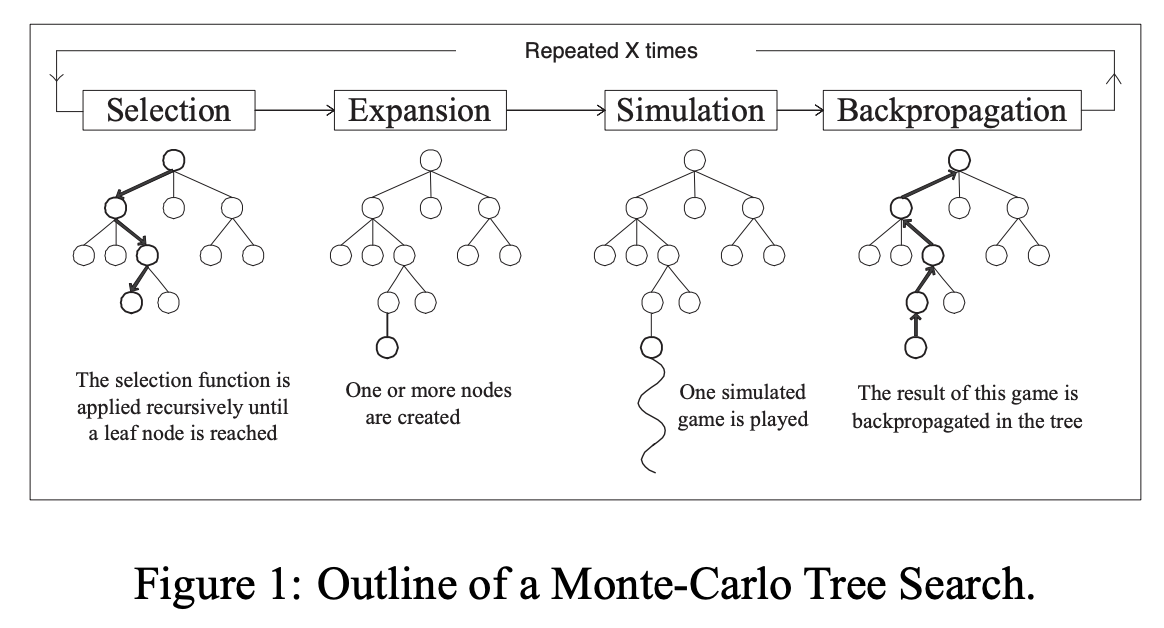
\includegraphics[width=0.75\textwidth]{Figures/MCTS.png}
	\caption{One iteration of a \acrshort{mcts} algorithm}
\end{figure}

\section{Model based \acrshort{mcts}}
\label{section:RL:ModelBasedMCTS}
While we explained how \acrshort{mcts} works in the previous section, some components were left without much discussion:
\begin{enumerate}
	\item The selection policy $\Pi^{\text{selection}}$
	\item The playout policy $\Pi^{\text{playout}}$
	\item Children creation
\end{enumerate}
This was deliberate, as the full power of $\acrshort{mcts}$ requires a good choice of the components, especially $\Pi^{\text{selection}}$ and $\Pi^{\text{playout}}.$

In our case, both functions will be based on the model $\mathcal{M}$ that we designed in chapter \ref{section:ModelDesign} and illustrated in figure \ref{fig:ModelArchitecture}.

Remember that our model $\mathcal{M}$ takes a \acrshort{mpg}\footnote{In fact, it takes a batch of \acrshortpl{mpg}, but this can be easily migitated.}, and produces two outputs:
\begin{enumerate}
	\item The predicted evaluation $v.$
	\item The predicted strategy $\Pi.$
\end{enumerate}
Both of these terms will be used in the \acrshort{mcts}.

\subsection{Create children}
In this version of \acrshort{mcts}, create children will return the list of all adjacent states. It does also apply an optional Dirichlet noise $\mathcal{D}(\alpha)$ if the current node is root.

\begin{algorithm}[H]
	\caption{Create children}\label{alg:CreateChildren}
	\begin{algorithmic}
		\Require $h$ current
		 node
		 \Require Dirichlet noise parameter $\alpha\in\mathbb{R}_+$
		 \Require Exploration noise parameter $\varepsilon\in[0,1]$
		 \Require Prior distribution $\Pi$
		\Ensure A list of children $C$
		\Ensure Optionally update $\Pi$
		\State $G=(V,E,W,s,p)$ is the underlying \acrshort{mpg} related to node $h$
		\State $m\leftarrow \lvert \Adj s \rvert$
		\If {$\text{root}(h)$}
			\State generate $\nu\sim \mathcal{D}(\alpha \ones_m)$ \Comment{$\ones_m \in \mathbb{R}^m$ is the vector of ones}
			\For {$(v,x)\in \zip(\Adj s,\nu)$}
				\State $\Pi(v)\leftarrow (1-\varepsilon)\Pi(v) + \varepsilon x$
			\EndFor
		\EndIf
		\State $C\leftarrow \varnothing$
		\For {$t\in \Adj s$}
			\State $G'\leftarrow (V,E,W,t,\bar{p})$
			\State $\text{append}(C,G')$
		\EndFor
		\State \Return $C$
	\end{algorithmic}
\end{algorithm}

\subsection{Playout Policy}
\label{section:RL:ModelBased:PlayoutPolicy}
In Alpha Zero's implementation of \acrshort{mcts} \cite{AlphaGo}, the playout policy is exactly the predicted distribution $\Pi.$

Also, the simulation algorithm \ref{alg:MCTSSimulation} was modified to only play one move:

\begin{algorithm}[H]
	\caption{Alpha Zero \acrshort{mcts} Simulation}\label{alg:AZSimulation}
	\begin{algorithmic}
		\Require $t$ the new child of the \acrshort{mcts}.
		\Require $\mathcal{M}$ the neural network model
		\Ensure $W$ the cumulative rewards after the playout for each player.
		\State  $G\leftarrow \text{MPG}(t)$ \Comment{get the current state}
		\State  $p\leftarrow \text{player}(t)$ \Comment{get the current player}
		\If {$p$ is $\Min$}
			\State $G\leftarrow \bar{G}$
		\EndIf
		\State $(v,\Pi)\leftarrow \mathcal{M}(G)$
		\If {$p$ is $\Min$}
			\State $v\leftarrow -v$
		\EndIf
		\State $W\leftarrow v$
		\Return $W$
	\end{algorithmic}
\end{algorithm}
\FloatBarrier
\subsection{Selection Policy}
\label{section:RL:ModelBased:SelectionPolicy}
\begin{algorithm}[H]
	\caption{model-based \acrshort{mcts} playout policy}\label{alg:SelectionPolicy}
	\begin{algorithmic}
		\Require $h$ current node 
		\Require $C\in\mathbb{R}_+$ exploration parameter
		\Ensure An child \acrshort{mpg} $G'$
		\State $Z\leftarrow \boldsymbol{0}$
		\For {$c\in \text{children}(h)$}
			\State $Z(c)\leftarrow \PUCT(c,h,\Pi(c),C)$
		\EndFor
		\State \Return $\displaystyle c \leftarrow \argmax_{c\in \text{children}(h)}Z(c)$
	\end{algorithmic}
\end{algorithm}
Here $\PUCT$ is defined as follow:
\begin{equation}
	\label{eqn:PUCT}
	\PUCT(c,h,\Pi(c),C) = H(c) + C\cdot \Pi(c) \cdot \frac{\sqrt{N(h)}}{N(c)+1}
\end{equation}
Here $H(c)$ is the reward of the current player at node $c$.

The equation \eqref{eqn:PUCT} was defined in the Alpha Go paper \cite{AlphaGo} as a model-based variant of $\UCT$ \cite{UCT}. We show the latter's expression to show the differnece between vanilla \acrshort{mcts} and model-based \acrshort{mcts}:
\begin{equation*}
	\UCT(c,h,C) =  H(c) + C\cdot \frac{\log {N(h)}}{N(c)+1}
\end{equation*}

In fact, the additional term $\Pi(c)$ is used to weight the children selection by the prior distribution $\Pi,$ and we believe that using the square root instead of the logarithmic function was deliberate to boost exploration.

\subsection{Wrapping up}
Our model-based \acrshort{mcts} is heavily inspired from the one used at Alpha Zero.

It uses the algorithm \ref{alg:MCTS} with a threshold number of iterations $N$ as exit condition\footnote{This applies to the model training phase. While deploying the algorithm, we can use a different exit condition.}. It avoids complete rollouts, and instead uses the simulation algorithm \ref{alg:AZSimulation} that uses the model $\mathcal{M}$.

Also, the predictions of model $\mathcal{M}$ are directly used in the selection policy defined at section \ref{section:RL:ModelBased:SelectionPolicy} and the playout policy defined at section \ref{section:RL:ModelBased:PlayoutPolicy}.
\subsection{Updating model}
Once the \acrshort{mcts} algorithm terminates. We get for each node a new estimates of both the strategy and the evaluation.
\subsubsection{Evaluation estimate}
The term $H$ used in the \acrshort{mcts} is used for the expected reward for the algorithm. Now as each node $t$ of the tree encodes a \acrshort{mpg} $G,$ $H(t)$ will be the updated estimate of the evaluation:
\begin{equation*}
	v(G)=\mathcal{M}(G)_{\text{evaluation}}
\end{equation*}

For that, we will denote the updated value as $v'(G)=H(t)$

\subsubsection{Strategy estimate}
To illustrate our point, we will need the following definitions:
\begin{itemize}
	\item Let $t$ be a node.
	\item Let $G=(V,E,W,s,p)$ be the \acrshort{mpg} encoded by $t.$
	\item Let $a\in \Adj s$ be an action eligible from $t.$
	\item Let $c$ be the\footnote{It is unique as an \acrshort{mpg} is deterministic. For a stochastic \acrshort{mpg}, which is out of the scope of this report, one should do a more careful analysis.} node resulting from applying $a$
\end{itemize}

Now, we want an esimtate of the strategy implied by the \acrshort{mcts}. In fact, the  term $N$ used for total explorations helps us to achieve this as following:
\begin{equation}
	\Pi'(G)(a) = \frac{N(c)}{N(t)} 
\end{equation}
Here, $\Pi'(G)$ will be the refined estimate of $\Pi(G)$

\subsubsection{Refitting}
\begin{itemize}
	\item Let $\Theta$ be the learnable parameters of $\mathcal{M}_\Theta=(v_{\Theta},\Pi_{\Theta})$
	\item Let $G^{(1)},\dots,G^{(m)}$ a batch of \acrshortpl{mpg}.
\end{itemize}
We will execute the \acrshort{mcts} on each game $G^{(i)}$ with the model $\mathcal{M}_{\Theta}$ to get a finer estimate of the evaluation $v'_{\Theta}(G^{(i)})$ and the strategy $\Pi'_{\Theta}(G^{(i)}).$

Once, we generate enough samples with \acrshort{mcts}. We train the model $\mathcal{M}_{\Theta}$ against $\mathscr{D}$ defined as follow:
$$
\mathscr{D}=\left[\left(G^{(1)},v'_{\Theta}(G^{(1)}),\Pi'_{\Theta}(G^{(1)})\right), \dots,\left(G^{(m)},v'_{\Theta}(G^{(m)}),\Pi'_{\Theta}(G^{(m)})\right)\right]
$$ 
The training uses the objective function defined on.

This will give us new learnable parameters $\Theta'$, and thus a new model $\mathcal{M}_{\Theta'}.$ With that, we will repeat the process indefinitively.


\section{Services}
\subsection{Rationale}
In section \ref{section:RL:ModelBasedMCTS}, we discussed our model-based implementation of \acrshort{mcts}. Roughly speaking, it can be divided into two main components that are repeated indefinitevely:
\begin{enumerate}
	\item Executing \acrshort{mcts} using model $\mathcal{M}_{\Theta^{(i)}}$ to generate a dataset $\mathcal{D}$: $$
	\mathscr{D}=\left[\left(G^{(1)},v'_{\Theta}(G^{(1)}),\Pi'_{\Theta}(G^{(1)})\right), \dots,\left(G^{(m)},v'_{\Theta}(G^{(m)}),\Pi'_{\Theta}(G^{(m)})\right)\right]
	$$
	\item Fit $\mathcal{M}_{\Theta^{(i)}}$ against $\mathscr{D}$ to get a better model $\mathcal{M}_{\Theta^{(i+1)}}$
\end{enumerate}

Each one of these steps is computationnally intensive. And for that, we will use the \text{seperation of concerns} principle to split them into distinct services.\footnote{This seperation, while not necessary, is benificial as it gives the freedom to scale the self-play pipeline.}
\subsection{Learner}
The learner, as its name suggests, is the service that trains the model $\mathcal{M}$ upon receiving enough samples from the actors\footnote{Which we will define in the next section.}

\subsection{Actor}
An actor, is a service designed for generating samples to the learner by playing agains itself using model-based \acrshort{mcts}

In contrast to the learner, which is unique by design. The self-play pipeline can have many actors, and this is required in our case as it accelerate the execution of the whole pipeline.

\subsection{Evaluator}
This service, is a third component that is used to evaluate the performance of model-based \acrshort{mcts} against a fixed player.

Like the actor, a self-play pipeline can have many evaluators, and this is also required in our case as it give performance metrics against a wide range of players.

Now, we defined the services and talked briefly about their relations. The figure below will describe the communication between the services:
\begin{figure}[H]
	\centering
	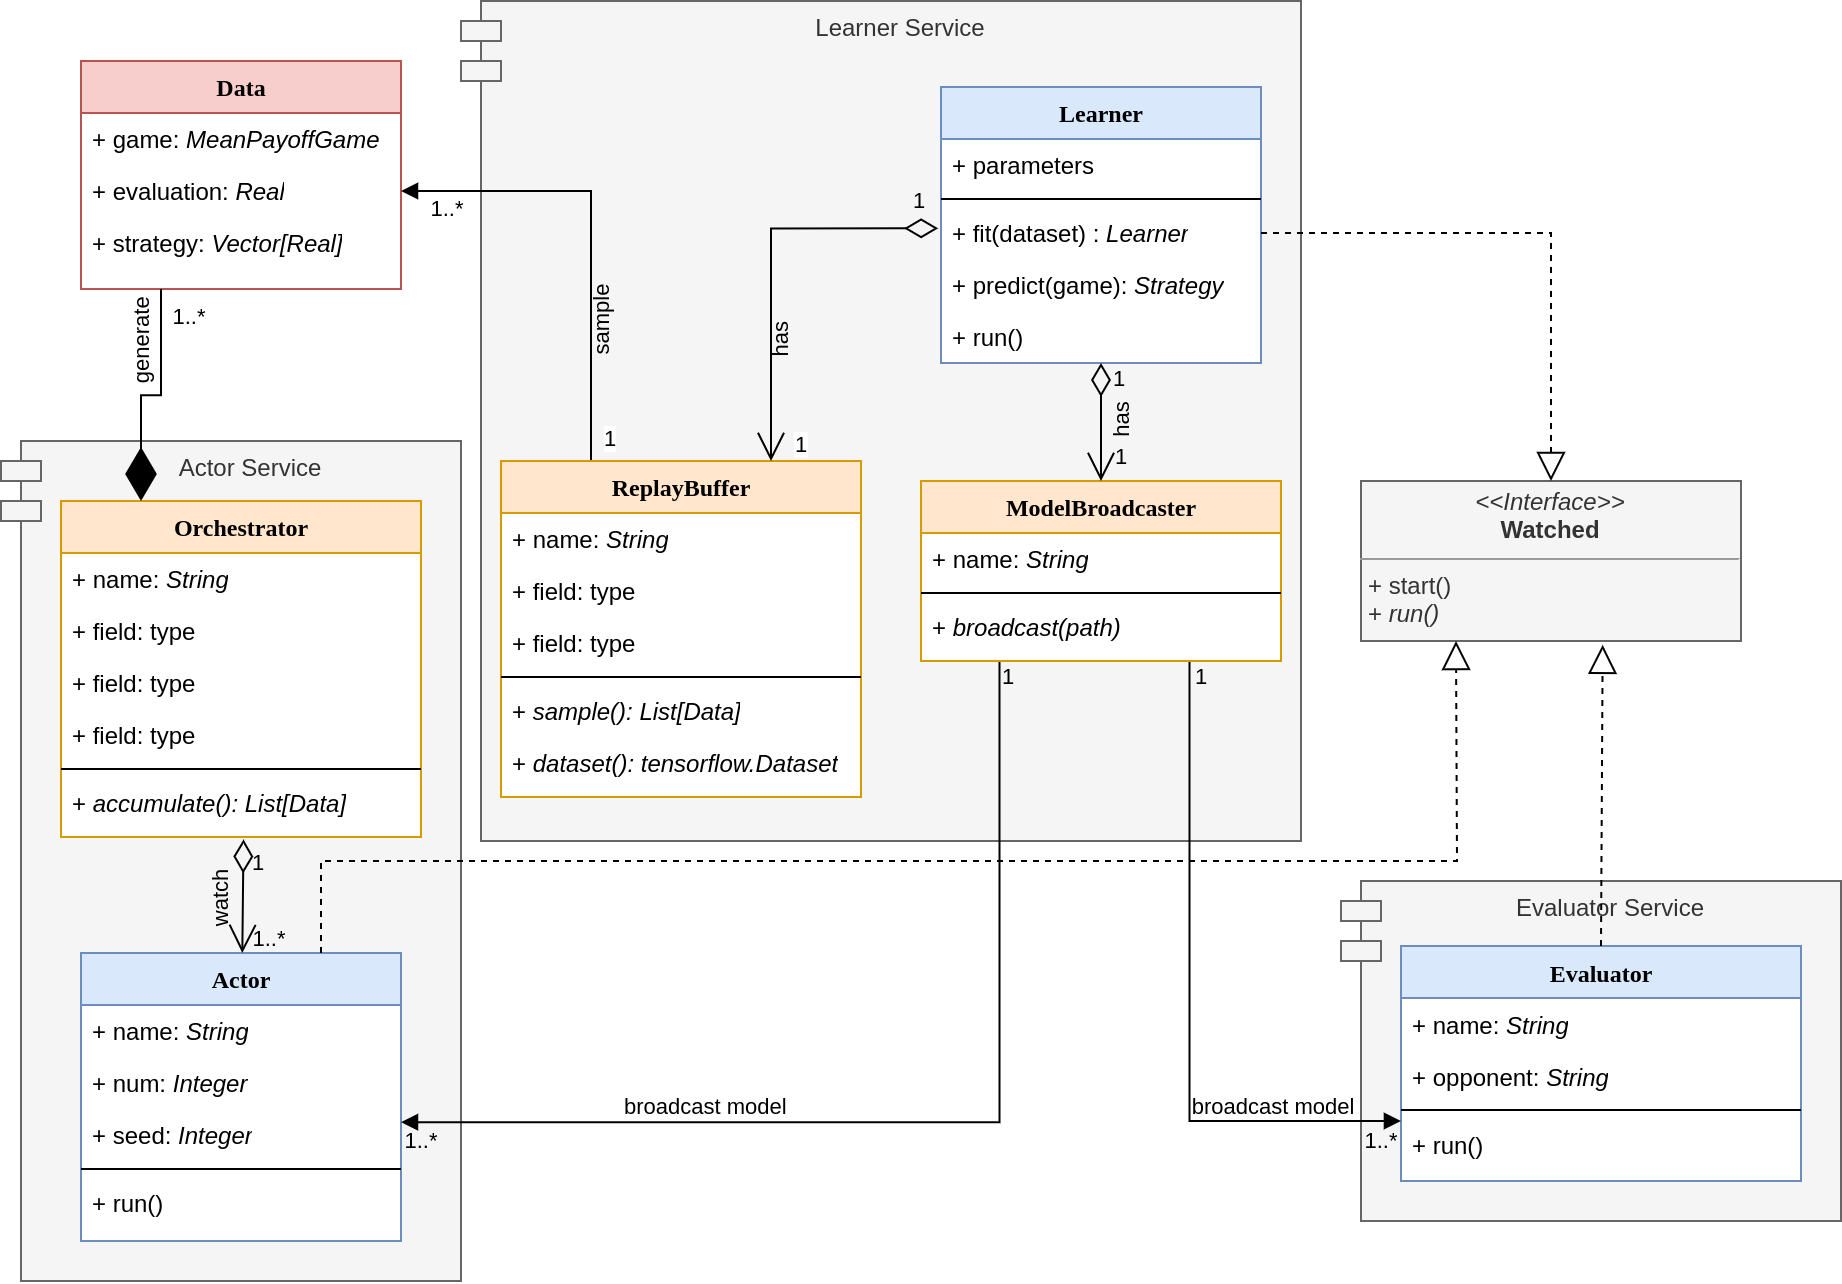
\includegraphics[width=0.7\textwidth]{Figures/ServiceRelations.png}
	\caption{Relation between different services\label{fig:RelationServices}}
\end{figure}
\FloatBarrier


\section{Self-play pipeline}
\subsection{Decoupling service communication}
In the previous section, we seperated logically between the different components of the self-play system.

Now, this seperation will give us the benefit of having multiple actors and evaluators per instance. While this is beneficial, it is only vertically scalable.

In fact, the interactions in figure \ref{fig:RelationServices} hints that the relation between components is tightly coupled. This is not the case, as we applied the \textbf{broker} design pattern to further decouple the communication between the different components of the system.

To do that, we introduced:
\begin{itemize}
	\item The \texttt{Orchestrator}: Which accumulate the generated annotated games and send them to the learner. It is a part of the actor service.
	\item The \texttt{ReplayBuffer}: Which loads a dataset from the annotated games that were generated by actors. It is part of the learner service.
	\item The \texttt{ModelBroadcaster}: It broadcast the new model to all actors and evaluators. It is part of the learner service.
\end{itemize}
The figure below details the relation between all main components of the pipeline:

\begin{figure}[H]
	\centering
	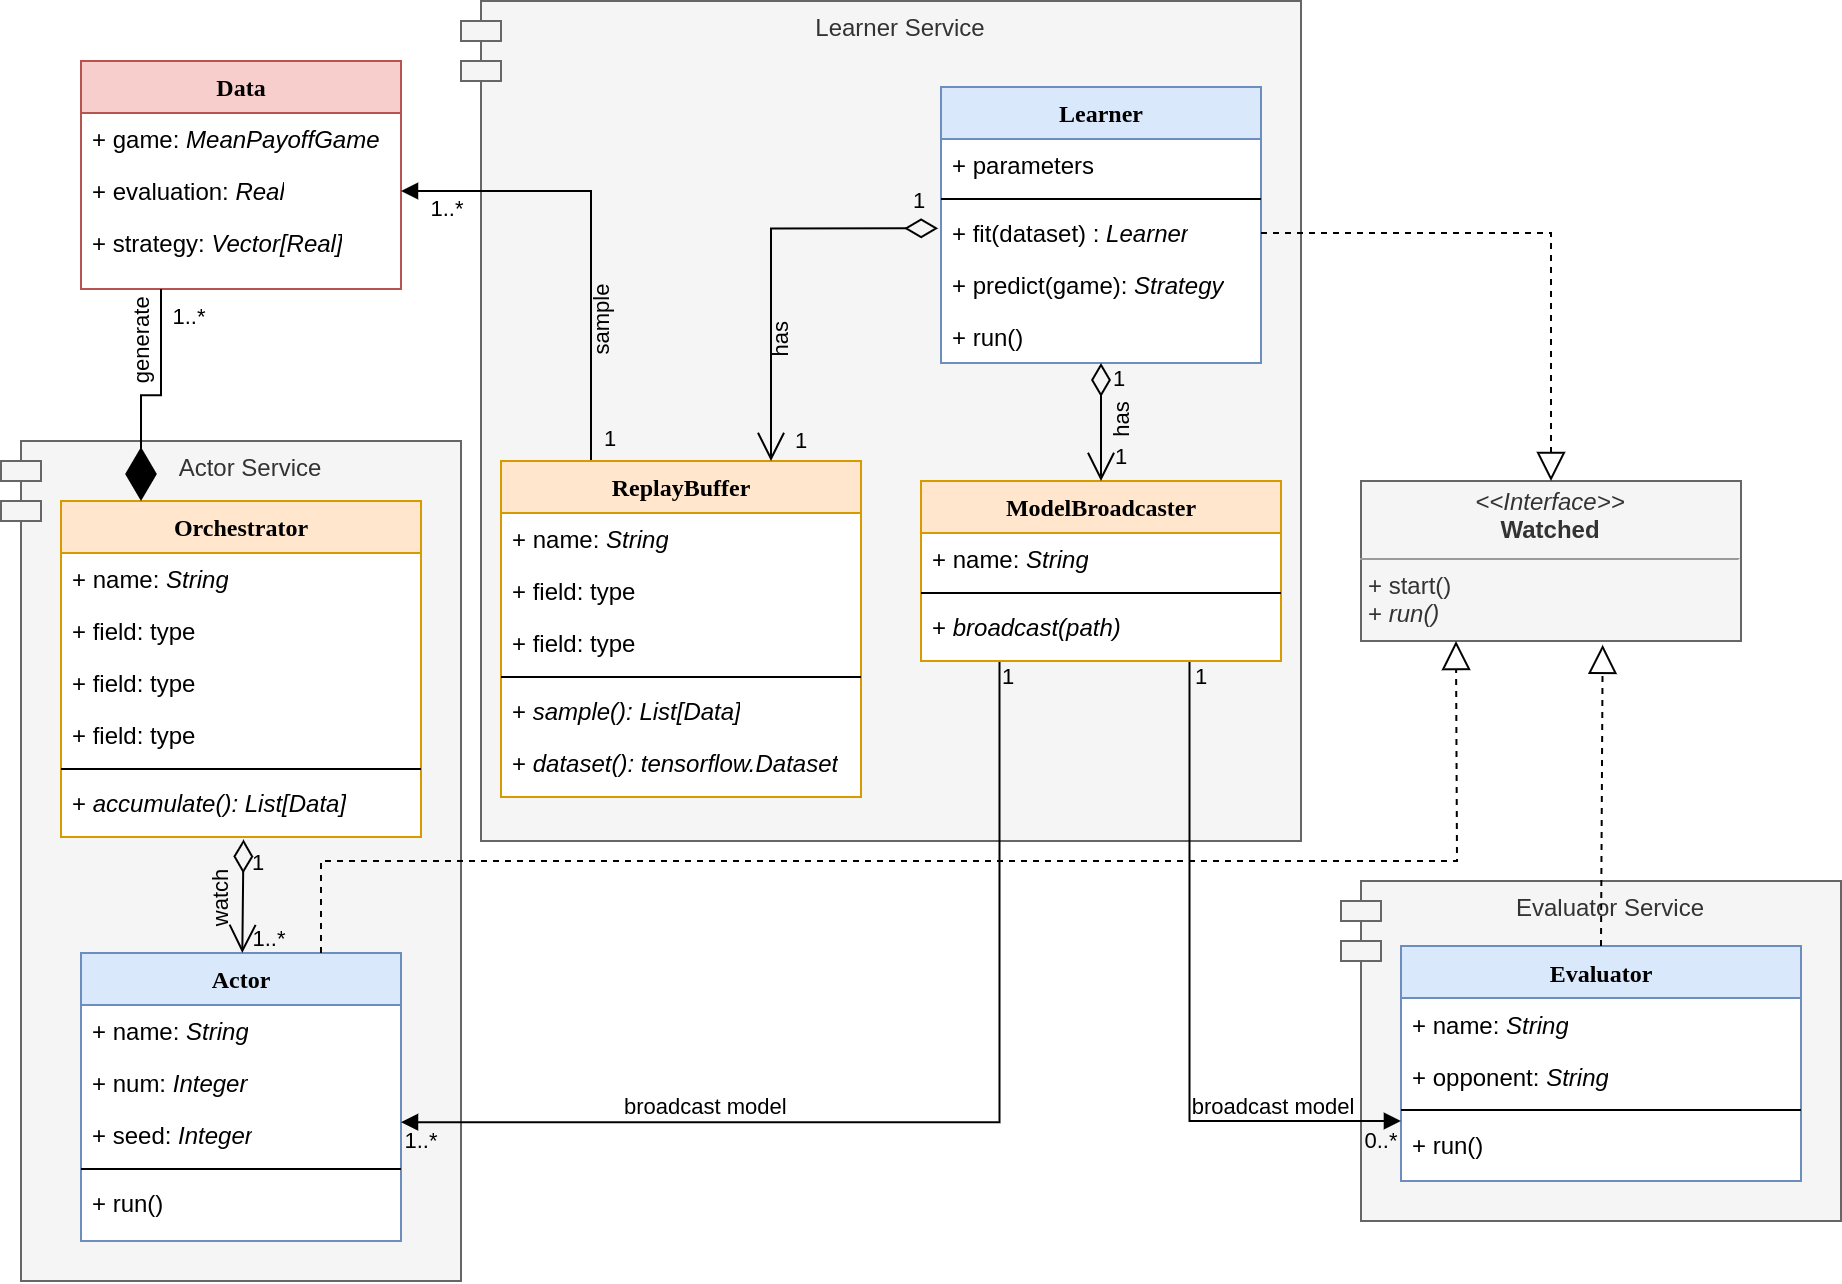
\includegraphics[width=0.85\textwidth]{Figures/ServiceDiagram.png}
	\caption{Class diagram of the services}
\end{figure}
\FloatBarrier
\subsection{Distributing the pipeline}
As we decoupled the communication, we only have to implement concrete definitions of the \texttt{Orchestrator}, \texttt{ReplayBuffer} and \texttt{ModelBroadcaster}.

Currently, we do have two set of implementations:
\begin{itemize}
	\item The first one defines the communication between the different services when they are centralized\footnote{Executed in the same machine.}.
	\item The second one defines the communication between the different services when they are distributed
\end{itemize}
The first implementation is present for compatibility reasons with the original implementation offered by \texttt{open\_spiel}. 

We distributed our pipeline by using the \acrshort{http} protocol\footnote{Note that this is not the only way to do that, the implementer is free to make his own implementation of \texttt{Orchestrator}, \texttt{ReplayBuffer} and \texttt{ModelBroadcaster}}. In fact, we used both \acrshort{rest} and \acrshort{grpc}.
Additionnally, both of \texttt{Orchestrator} and \texttt{ReplayBuffer} use \acrshort{grpc}, while \texttt{ModelBroadcaster} uses \acrshort{rest}. This will give us the opportunity to add horizontal scaling for the pipeline, by adding further actor nodes\footnote{Here node refers to a machine.} and evaluator nodes.

The next two sections are dedicated respectfully to the \acrshort{rest} server and the \acrshort{grpc} server.
\subsection{\acrshort{rest} servers}
Each service\footnote{Either actor or learner or evaluator} deploys a basic \textbf{FastAPI} \acrfull{rest} server used mainly for: 
\begin{itemize}
	\item Basic management: starting the pipeline or shutting the pipeline.
	\item Service discovery.
	\item Model broadcasting.
	\item Monitoring.
\end{itemize}
The learner actor serves as the master of the services. It will give instructions to the other services. It also serves as the gateway.

\begin{table}[h]
	\begin{tabularx}{\textwidth}{| p{3cm} | p{1.2cm} | p{1.7cm} | X |}
		\hline
		Route & Method & Service & Description \\
		\hline 
		\texttt{/start} &  GET & All & If the service is the learner, start the whole pipeline by requesting \texttt{/start} to all other services. Otherwise, start the requested service. \\
		\hline
		\texttt{/stop} &  GET & All & If the service is the learner, stop the whole pipeline by requesting \texttt{/stop} to all other services. Otherwise, stop the requested service. \\
		\hline
		\texttt{/heartbeat} & GET & All & Return a heartbeat. \\
		\hline
		\texttt{/replay\_buffer} & GET & Learner & Ouput information in JSON format about the \newline \textbf{Reverb} server. \\
		\hline
		\texttt{/config} & GET & Learner & Ouput the configuration file in JSON format. \\
		\hline
		\texttt{/discovery} & GET & Learner & Discover the services. \\
		\hline
		\texttt{/model} & POST & Actor, Evaluator & Sends the path of the newest version of the model. \\
		\hline
		\texttt{/stats} & GET & Actor, Evaluator & Manually get the statistics generated by the service.\\
		\hline
	\end{tabularx}
	\caption{Supported routes
		\label{table:ImplementedRoutes}}
\end{table}

\subsection{\acrshort{grpc} server}
The learner service also deploys a \textbf{Reverb}\footnote{Reverb is an efficient data storage and experience replay system for distributed reinforcement learning. It supports multiple data structure representations such as FIFO, LIFO, and priority queues. } server, which we will use for storing annotated games and sampling from them. It is based on \acrfull{grpc}\footnote{This is a recursive acronym.}, and designed primarly for efficiency. 

\begin{figure}[H]
	\centering
	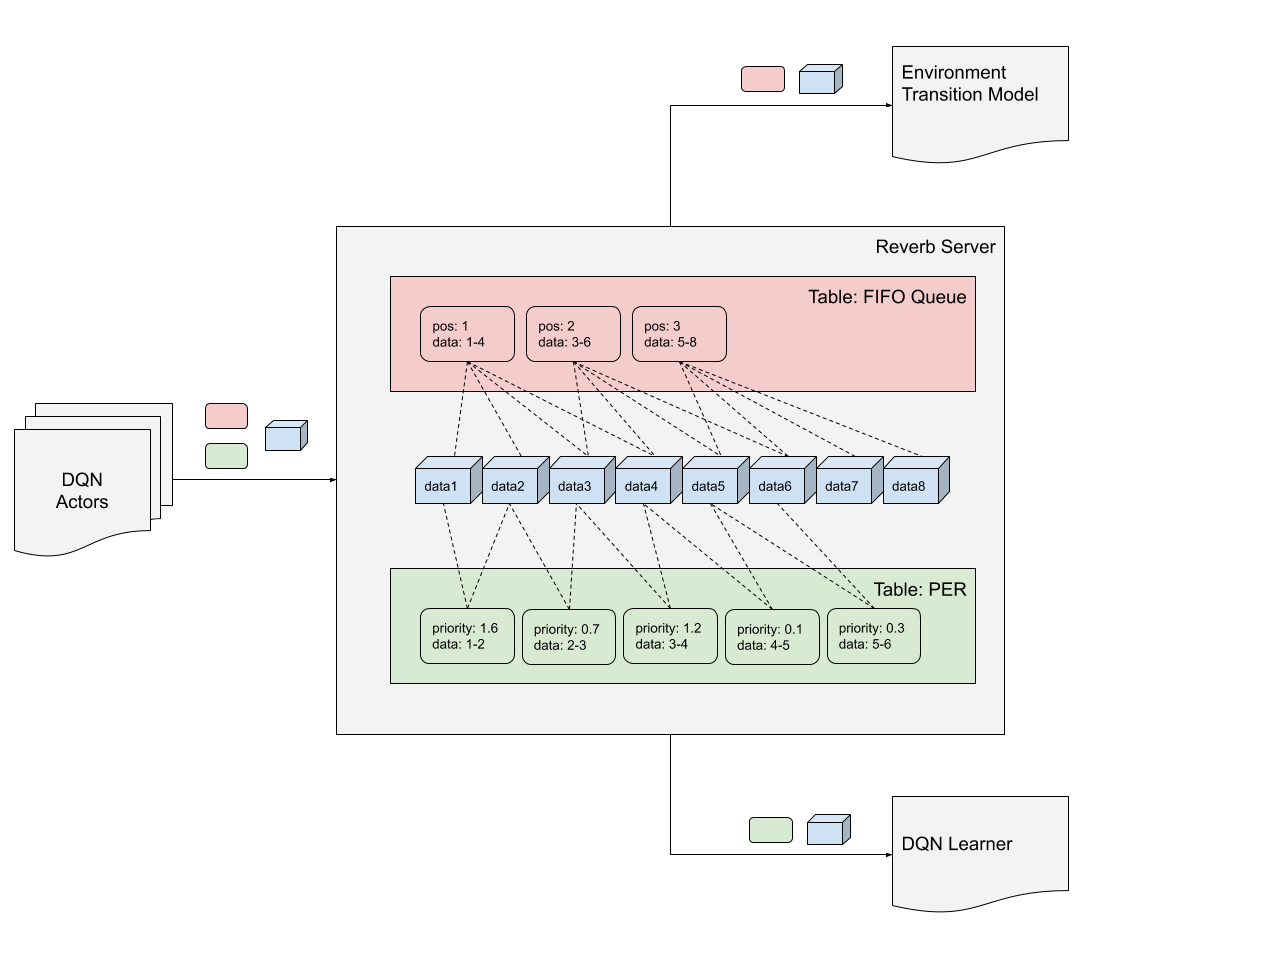
\includegraphics[width=0.9\textwidth]{Figures/ReverbTable.png}
	\caption{Illustration of how Reverb works}
\end{figure}
\FloatBarrier
This server will act as an intermediate between the actors and the learner in the following sense:
\begin{itemize}
	\item The implemented \texttt{Orchestrator} will send batches of generated games to the server.
	\item The implemented \texttt{ReplayBuffer} will take samples from the \textbf{Reverb} server for training purposes.
\end{itemize}

\subsection{Tensorboard server}
\section{Implementation}

\section{Deployment}


\begin{figure}
	\centering
	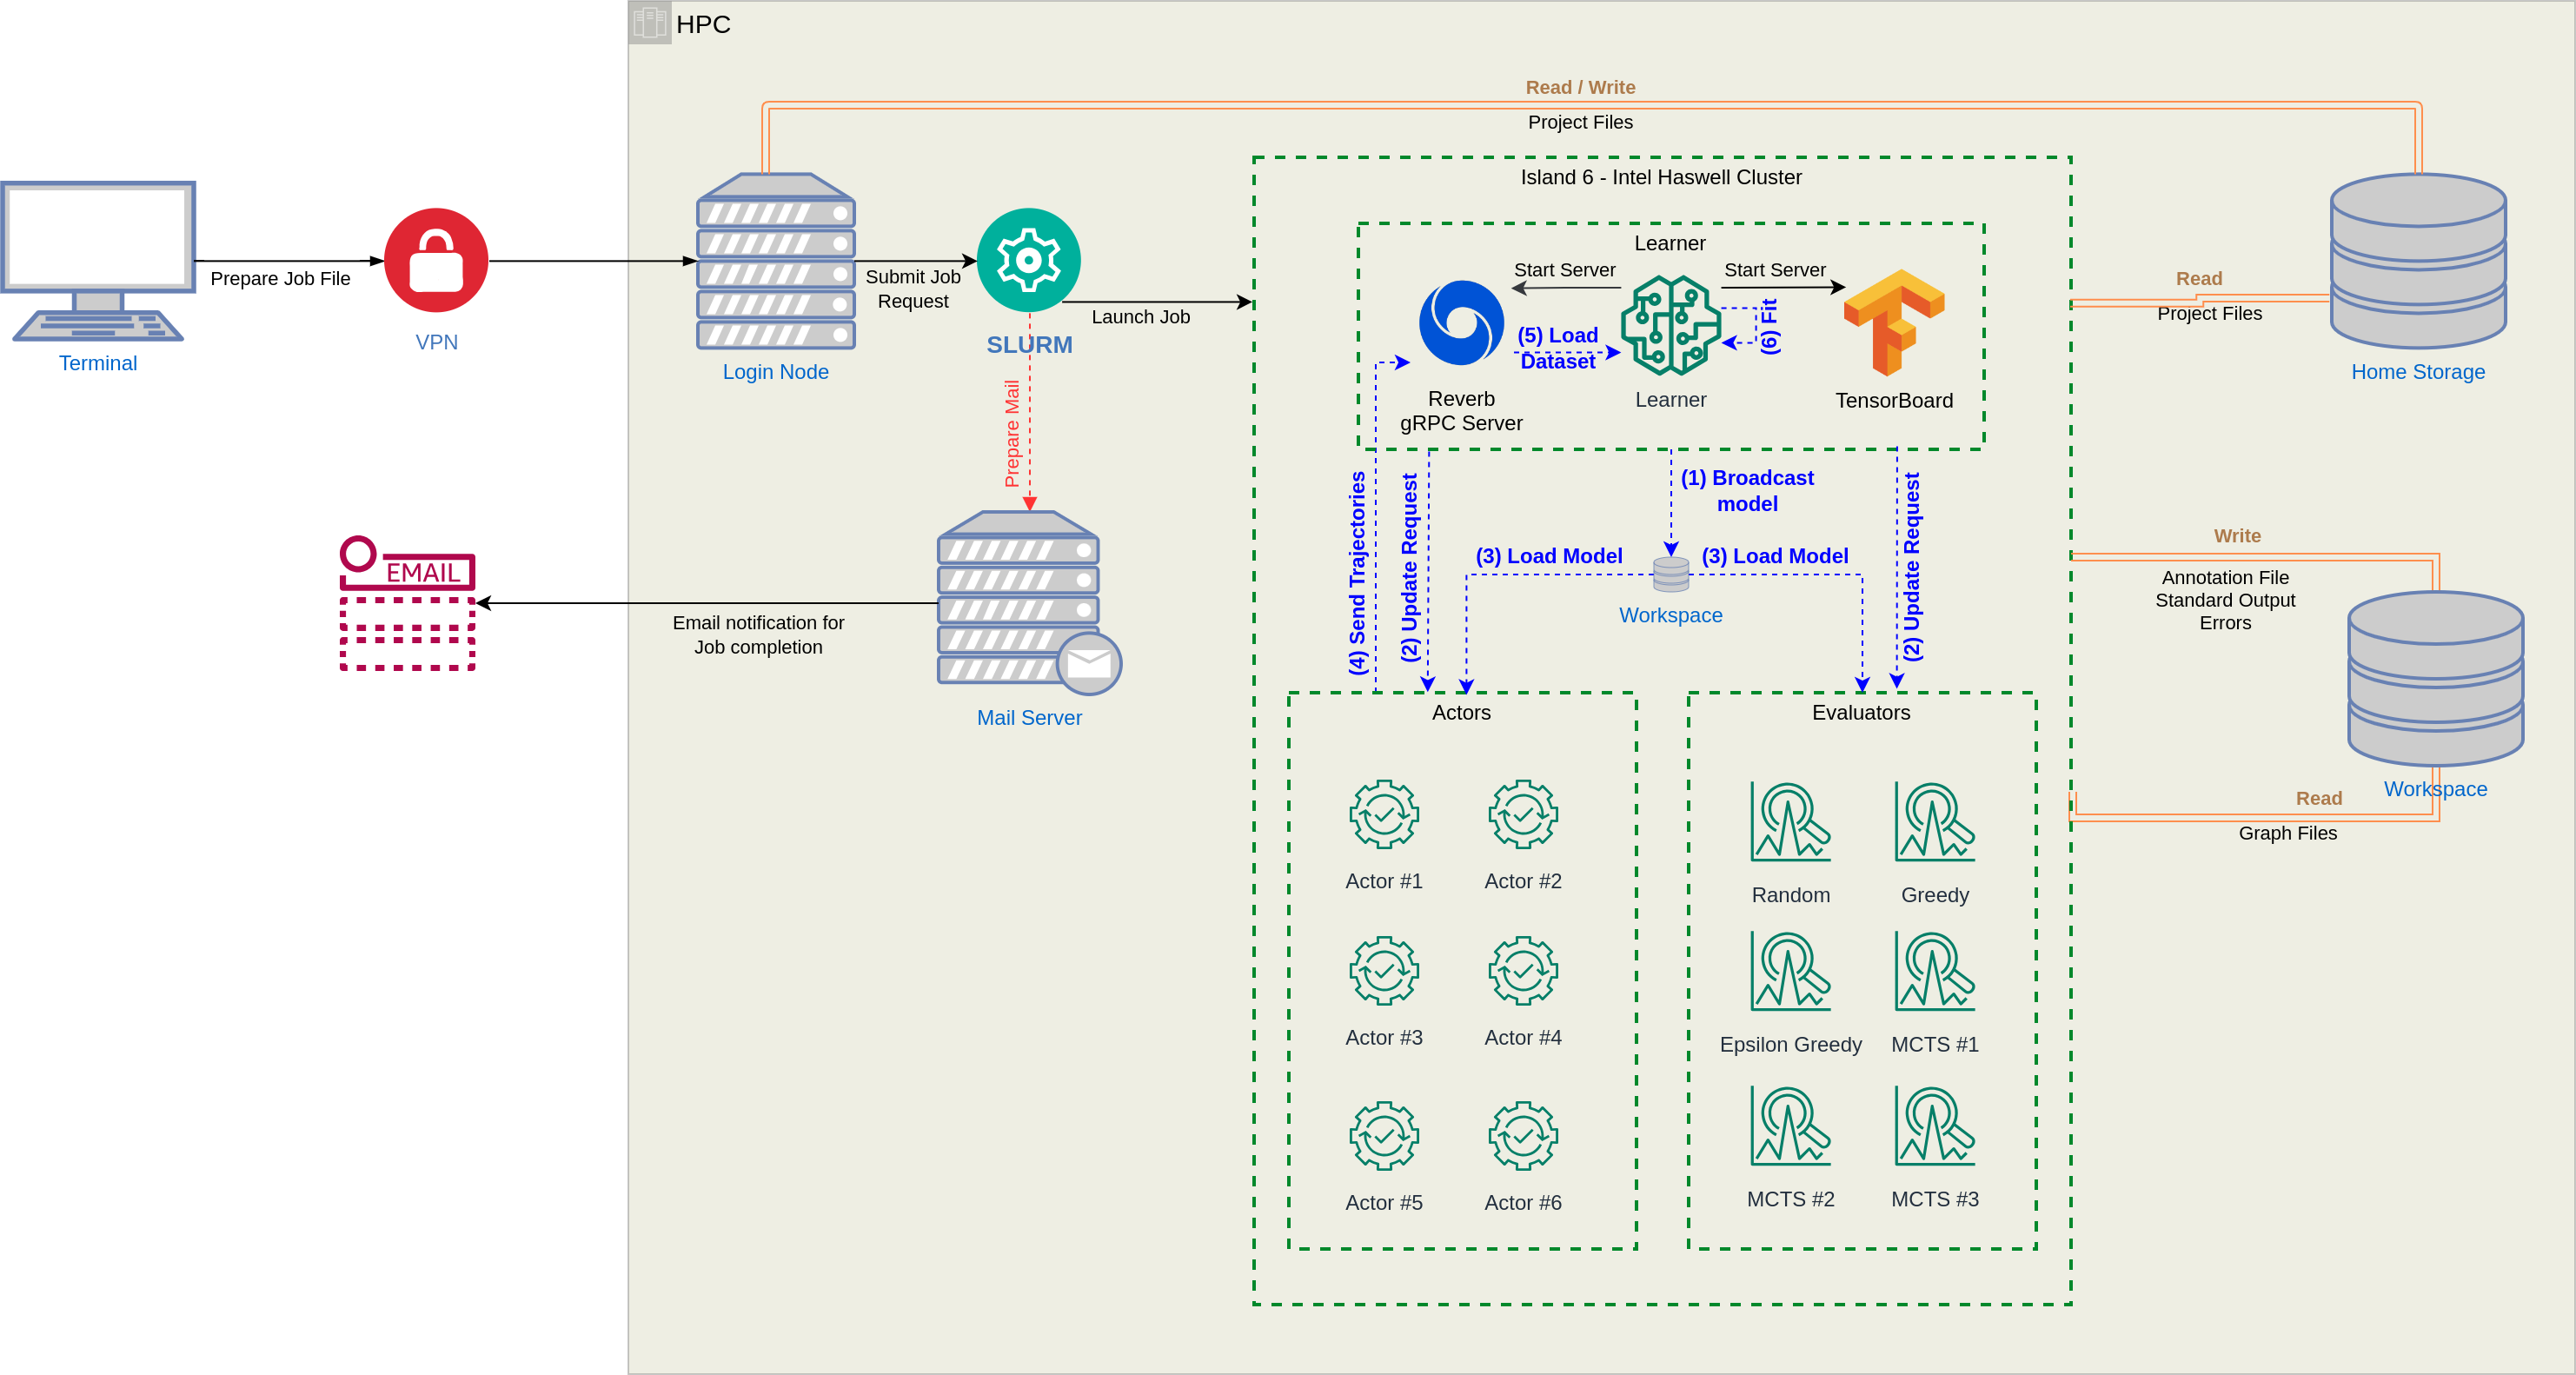
\includegraphics[width=0.95\textwidth]{Figures/AlphaZero.png}
	\caption{Pipeline Architecture}
\end{figure}
\section{Configuration}
We externalized the configuration of our self-play pipeline, so that we could change the parameters and fine-tune the hyper-parameters without modifying the source code\footnote{Still, the pipeline needs to be restarted for changes to take effect.}. This gives us the possibility to play experiments until getting the desired computational and prediction performances.

We created a \acrshort{yaml} configuration file with the name \texttt{configuration.yml} that we already introduced in section \ref{section:ModelDesign:Configuration}. It will be used by all services\footnote{In a future iteration, we plan to split this file per service.}. When we completed the externalization process, we found out that we need also to set the file as a template so we can change it dynamically by environment variables. This is beneficial as we do have many instances of the same services that only differ by some minor hyper-parameters.

To achieve this, we introduced \textbf{Jinja} templating into the file, and set the name of the template configuration file as \texttt{configuration.yml.j2}. The templated configuration variables includes:
\begin{itemize}
	\item \texttt{path}: The directory of the pipeline
	\item The instance name of the service.
	\item The port used by the services \acrshort{rest} server.
	\item Type of the opponent for an evaluator service.
	\item The address and port of the \acrshort{grpc} service.
\end{itemize}

In the remaining of this section, we will describe the remaining configurations except the training and model configurations as they were already discussed in figures \ref{fig:ModelConfiguration} and \ref{fig:TrainingConfiguration}.

\subsection{Replay buffer}
Our pipeline supports two kinds of replay buffer. A ``\texttt{local}" one, that we can use in a centralized system. And a ``\texttt{grpc}" one\footnote{Which is the \textbf{Reverb} server.}, which is the one we are using.

The figure below shows the configuration parameters of the replay buffer:
\begin{figure}[ht]
	\centering
	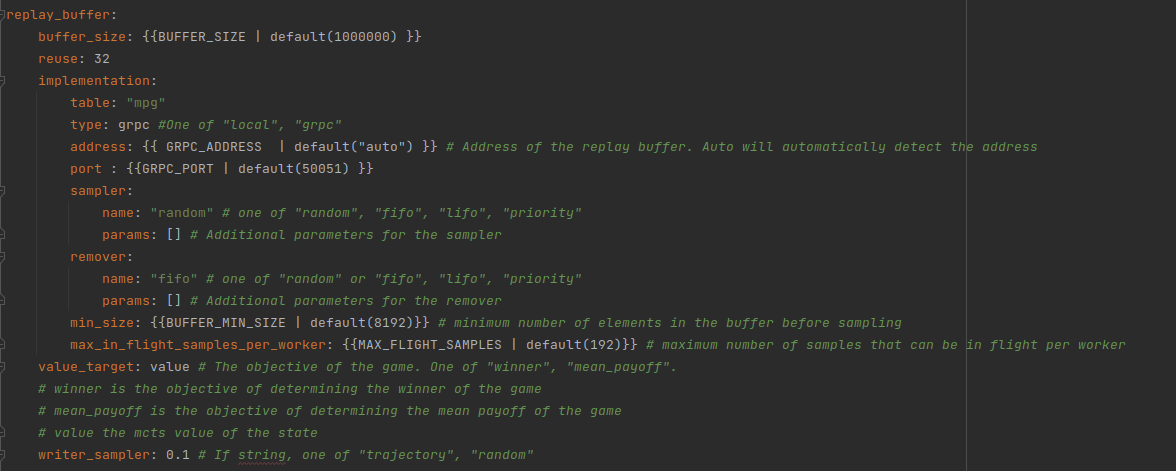
\includegraphics[width=0.95\textwidth]{Figures/ReplayBufferConfiguration.png}
	\caption{Replay buffer section of the configuration file \label{fig:ReplayBufferConfiguration.png}}
	\small{Note: while this is a recent version of the configuration file, we may tweak it further for fine-tuning purposes.}
\end{figure}
\FloatBarrier
%
\subsection{Services}
We also externalized the parameters of the services, so we can easily change their depoloyment options. This is shown by the figure below:
\begin{figure}[ht]
	\centering
	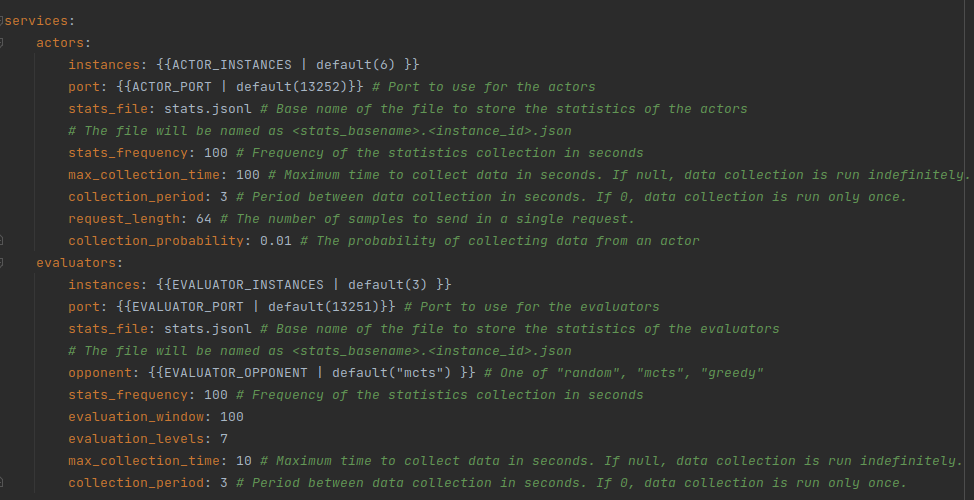
\includegraphics[width=0.95\textwidth]{Figures/ServicesConfiguration.png}
	\caption{Replay buffer section of the configuration file \label{fig:ServicesConfiguration.png}}
	\small{Note: while this is a recent version of the configuration file, we may tweak it further for fine-tuning purposes.}
\end{figure}
\FloatBarrier
\section{Execution}